\documentclass[english]{article}
\usepackage[T1]{fontenc}
\usepackage[utf8]{inputenc}
\usepackage[catalan]{babel}
\usepackage{lmodern}
\usepackage{microtype}
\usepackage{graphicx}
\usepackage{babel,blindtext}
\usepackage{geometry}
\usepackage{amsmath}
\usepackage{framed}
\usepackage[font=footnotesize,labelfont=bf]{caption}
 \geometry{
 a4paper,
 total={170mm,257mm},
 left=20mm,
 top=20mm,
 }

\begin{document}
\newcommand\makeAbstract{%
\begin{center}\textbf{Abstract (versió en català)}\end{center}
\begin{list}{}{\leftmargin=3em\rightmargin=\leftmargin}\item\relax
\small
L'anàlisi de dades d'expressió genètica és un dels grans reptes estadístics per a detectar expressions diferencials entre gens sota una condició donada. La idea principal d'aquest treball, és la creació d'un protocol d'anàlisi interactiu de matrius d'expressió genètica. Es presenten mètodes estadístics com l'anàlisi de la variància (ANOVA). Mètodes de correcció per multiplicitat de contrastos també queden descrits. S'utilitzen mètodes gràfics com els mapes de calor. Tot aquest protocol d'anàlisi s'implementa en una aplicació web desenvolupada amb Shiny.
\end{list}\par\vspace{6mm}%
\begin{center}\textbf{Abstract (versión en castellano)}\end{center}
\begin{list}{}{\leftmargin=3em\rightmargin=\leftmargin}\item\relax
\small
El análisis de datos de expresión genética es uno de los grandes retos estadísticos para detectar expresiones diferenciales entre genes mediante una condición establecida. La idea principal de este trabajo, es la creación de un protocolo de análisis interactivo de matrices de expresión genética. Se presentan métodos estadísticos como el análisis de la varianza (ANOVA). Métodos de corrección por multiplicidad de contrastes también quedan descritos. Se utilizan métodos gráficos como los mapas de calor. Todo este protocolo de análisis se implementa en una aplicación web desarrollada con Shiny.
\end{list}\par\vspace{6mm}%
\begin{center}\textbf{Abstract (English version)}\end{center}
\begin{list}{}{\leftmargin=3em\rightmargin=\leftmargin}\item\relax
\small
 Data gene expression analysis is one of the major statistical challenges to detect differential expressions between genes under a given condition. The main idea is the creation of an interactive analysis protocol of gene expression matrix. Methods are presented for detecting differential expression using statistical hypothesis testing methods including analysis of variance (ANOVA). Methods for multiple testing correction and their application are described. Graphical methods such as heatmaps are used. This analysis protocol is implemented in a web application developed in Shiny.
\end{list}\par\vspace{6mm}%
}

\title{
\textsc{Treball de final de grau}\\[2.6cm]
{\LARGE \bfseries Protocol d'anàlisi per a dades d'expressió gènica amb Shiny}\\{\Large\bfseries Grau d'Estadística Aplicada}\\[5cm]
}

\author{
\textsc{Autor:} Antonio Rodríguez Gómez
}

\date{
\textsc{Supervisor:} Mercè Farré \\[1em]
\today
}

\maketitle
%%% Local Variables:
%%% mode: latex
%%% TeX-master: "test"
%%% End:

\thispagestyle{empty}
\clearpage
\twocolumn[\makeAbstract]
\thispagestyle{empty}
\clearpage
\tableofcontents
\clearpage
\section{Introducció}
Un dels reptes més grans de la biologia actualment és analitzar els volums massius de dades creats, per exemple, en la seqüenciació de DNA. La gran evolució de les tècniques de recollida de dades biològiques ha fet que sigui necessari el desenvolupament de metodologies eficients a l'hora de tractar i analitzar les dades. La disciplina que recull aquestes metodologies s'anomena bioinformàtica.
\\

La bioinformàtica és un àrea emergent interdisciplinària que s'ocupa de l'aplicació de l'informàtica a la recopilació, emmagatzematge, organització, anàlisis, manipulació, presentació y distribució d'informació relativa a les dades biològiques o mèdiques.
\\

Aquest treball s'ha centrat en l'anàlisis de bases de dades d'expressió genètica a partir de diferents condicions experimentals. Al llarg del treball s'utilitzen técniques per analitzar aquests tipus de dissenys on l'objectiu recau en veure quins gens s'expressen significativament sota condicions experimentals establertes.
\\

Amb aquesta premissa, el treball també s'ha enfocat en crear un aplicatiu web capaç de fer un anàlisi estadístic de les matrius d'expressió gènica. L'aplicatiu ha sigut programat amb R, per mitjà del paquet Shiny. Aquest paquet és capa\c{c} d'implementar el codi R de manera interactiva. No només implementa el codi R, sinó també és capaç d'interactuar amb diferents llenguatges com html, css o java. Tot el conjunt de l'aplicació ha sigut organitzada i compartida per mitjà d'un repositori creat en la plataforma GitHub. D'aquesta manera el codi queda a disposició de qualsevol usuari que vulgui utilitzar-lo o consultar els métodes empleats.

\subsection{Introducció als conceptes bàsics de la bioinformàtica}
%(PDF de bioinformatica)(ttp://masteres.ugr.es/moea/pages/curso201314/tfm1314/tfm-septiembre1314/memoriamasterdanielparrasburgos/!)

Cada organisme es defineix pel seu material genètic, el genoma. La informació genètica la trobem emmagatzemada en una macromolècula anomenada DNA, que es troba al nucli de cada cèl·lula.
\\

Un gen consisteix en un segment de DNA que conté el codi per a la producció d'una proteïna. Una única cadena d'ADN conté milers de gens, cadascun sintetitza una proteïna concreta. Per fer-nos a la idea, els humans tenim al voltant de 20.000 gens. La longitud i seqüència d'un gen determina la grandària i la forma de la proteïna que sintetitza i quina funció tindrà aquesta proteïna dins de l'organisme.
\\

La dotació de gens que presenta una espècie, s'anomena genotip, i l'aparen\c{c}a externa d'un caràcter genètic, l'anomenem fenotip. L'expressió del genotip ve determinat, a més de per la càrrega genètica, per l'ambient i el comportament dels éssers vius. Si un gen no s'expressa en un individu, aquest tindrà el mateix fenotip que un individu que no presenti el gen. Però com podem arribar a obtenir una mesura de l'expressió dels gens? Existeixen tècniques per quantificar-ho? La resposta és sí.
\\

La mesura de l'expressió gènica generalment és dur a terme quantificant els nivells de producte del gen. Una tècnica molt utilitzada de mesura de l'expressió gènica que utilitza ARN missatger és la denominada transcripció inversa, seguida de la reacció en cadena quantitativa de la polimerasa (qPCR \footnote{Aquesta tècnica serveix per amplificar un fragment d'ADN i la seva utilitat rau en el fet que després de l'amplificació resulta molt més fàcil identificar material genètic amb una gran precisió.}). Una de les seves principals característiques és la seva sensibilitat, ja que només necessita una única molècula per iniciar el procés de replicació. A més, és molt robusta gràcies al fet que permet utilitzar diferents productes biològics, com cabells, teixits, mucoses, sang, etc. Aquesta tècnica és fonamental per l'anàlisi de dades d'expressió gènica, perquè per l'obtenció d'aquestes dades es requereix una quantitat suficientment gran de producte biològic que no sempre és de fàcil obtenció, per tant, és important disposar d'una tècnica que faciliti la seva replicació de forma controlada, robusta i eficient.
\\

Centres de genòmica s'encarreguen de fer aquests processos i de retornar els resultats en matrius de dades on es recullen els nivells d'expressió per a cada gen. Per tant, és important fer un bon disseny experimental ja que aquests procesos són costosos i requereixen de temps, a més del biaix estadístic que es pot generar.


\subsection{Cas d'estudi: Protocol d'análisi d'un OpenArray}
Des de la facultat de veterinaria de l'Universitat Autònoma s'han dut a terme estudis experimentals sobre l'expressió dels gens animals en certes condicions experimentals. L'aplicatiu web ha sigut creat per donar suport estadístic al grup d'investigació de la UAB \textbf{Nombre del grupo}.
\\

El cas d'estudi que el treball ha contemplat consisteix en un experiment amb animals, concretament, amb porcins. Durant l'experiment s'administraven diferents tractaments/dietes als porcins. D'aquesta manera es volia veure l'afectació d'alguns tractaments en la regulació intestinal i com afectava al creixement dels porcins.
\\

Les dades utilitzades en aquest treball han sigut proporcionades per \textbf{Nombre del grupo} per mitjà de la tecnologia OpenArray. El material biològic que s'ha utilitzat per l'obtenció de les dades, han sigut diferents tipus de teixits del intestí. Els gens van ser escollits amb criteris científics pels investigadors i tenen un significat concret dins del funcionament de la regulació intestinal.
\\

Encara que l'aplicatiu web s'ha creat a partir d'aquest estudi, la idea ha sigut generalitzar el codi per poder utilitzar-ho amb altres dissenys experimentals.

\section{Protocol d'anàlisi}
%https://stats.stackexchange.com/questions/78920/mathematical-explanations-behind-anova
En aquest apartat queden definits els mètodes estadístics utilitzats en el protocol d'anàlisi. Cada mètode ha sigut implementat en l'aplicatiu i més endavant es mostren els resultats del cas d'estudi.
\subsection{Anàlisi de la variància (ANOVA)}
L'anàlisi de la variància (ANOVA) és el mètode clàssic per comparar mitjanes entre grups dos grups o més. Suposem que tenim $N$ observacions repartides en $k$ grups i definim $n=\frac{N}{k}$. Llavors $x_{ij}$ seria l'individu $j$ corresponent al grup $i$. En aquest cas assumim que l'estudi és balancejat, és a dir, el nombre d'individus per grup és el mateix. Denotem $\bar{x.}$ com la mitjana de la mostra global, i $\bar{x_{i}}$ com la mitjana del grup $i$.
Les observacions es poden tornar a escriure com:
\begin{equation*}
x_{ij} = \bar{x.} + (\bar{x_{i}} - \bar{x.}) + (x_{ij} - \bar{x_{i}})
\end{equation*}
Això ens porta al següent model:
\begin{equation*}
x_{ij} = \mu + \alpha_{i} + \epsilon_{ij}
\end{equation*}
on $\mu$ i $\alpha_{i}$ són la mitjana global i la mitjana del grup $i$ respectivament. S'assumeix que el terme d'error $\epsilon_{ij}$ és iid i segueix una distribució normal
\begin{equation*}
\epsilon_{ij} \sim \mathcal{N}(\mu,\,\sigma^{2})\,
\end{equation*}
La hipòtesi nul·la en un model ANOVA és que les mitjanes dels grups són iguals, és a dir:
\begin{equation*}
\alpha_1 = \alpha_2 = ... = \alpha_k
\end{equation*}
Si això és cert, el terme d'error per a la diferència de grups queda definit com:
\begin{equation*}
\bar{x_{i}} - \mu \sim \mathcal{N}(0,\,\frac{\sigma^{2}}{n}=\bar{\sigma}^2)\,
\end{equation*}
Es pot mesurar la quantitat total de variabilitat entre observacions sumant els quadrats de les diferències entre cadascun $\bar{x}.$ i $x_{ij}$:

\begin{equation*}
SST(\text{Suma de quadrats totals}) = \sum_{i=1}^{k} \sum_{j=1}^{n_{i}} (x_{ij} - \bar{x}.)^2
\end{equation*}
La variabilitat total es pot desglossar en 2 termes:
\begin{enumerate}
\item La variabilitat entre grups:
\begin{equation*}
SSG = \sum_{i=1}^{k} n_{i}(\bar{x}_{i} - \bar{x}.)^2
\end{equation*}
amb $k-1$ graus de llibertat.
\item La variabilitat intra grups:
\begin{equation*}
SSE = \sum_{i=1}^{k} \sum_{j=1}^{n_{i}} (x_{ij} - \bar{x_{i}})^2
\end{equation*}
amb $N-k$ graus de llibertat.
\end{enumerate}
Per tant, podem escriure la suma de quadrats totals com:
\begin{equation*}
SST = SSG + SSE
\end{equation*}

Si la variabilitat entre grups és gran en relació amb la variabilitat intra grups, llavors les dades suggereixen que les mitjanes de les poblacions són significativament diferents. Si no existeixen diferencies, entre els grups, esperaríem que les mitjanes quadràtiques
\begin{equation*}
MSG = \frac{SSG}{(k-1)}
\end{equation*}
\begin{equation*}
MSE = \frac{SSE}{(N-k)}
\end{equation*}
siguin similars. El test estadístic ANOVA es defineix com la ràtio entre les dues mitjanes quadràtiques:
\begin{equation*}
F = \frac{MSG}{MSE}
\end{equation*}
L'estadístic $F$ segueix una distribució F de Snedecor amb $k-1$ i $N-k$ graus de llibertat. Si la hipòtesi nul·la és certa, $F$ seria proper a 1. D'altra banda, si la mitjana quadràtica entre grups $MSG$ és gran, suposaria un valor gran de l'estadístic F. Bàsicament, l'ANOVA examina les dues fons de la variància total i mira quina part contribueix més. Per aquest motiu, s'anomena anàlisi de la variància encara que la intenció sigui comparar les mitjanes dels grups.
\\

Hi ha una sèrie de supòsits que s'han de fer abans que s'apliqui l'ANOVA, la desviació en aquests supòsits portaran a resultats que poden ser enganyosos o inexactes. Aquests supòsits inclouen la independència, normalitat i variància constant dels errors. En algunes situacions, hi ha transformacions que poden ser
utilitzades per evitar les violacions d'aquests supòsits, com ara la transformació logarítmica de les dades.

\subsubsection{Anova per a dissenys desbalancejats}
En procés...
\clearpage

\subsection{Correcció per multiplicitat de contrastos}
%http://www.stat.cmu.edu/~genovese/talks/hannover1-04.pdf
%Limma
Un problema comú què ens podem trobar a qualsevol investigació és voler comparar més de 2 grups de dades per detectar possibles diferències entre ells. La utilització de models d'ANOVA ens pot permetre detectar diferències, a escala global, entre les mitjanes involucrades, però en moltes ocasions volem detectar les diferències entre grups concrets. Aquest cas només és possible mitjançant l'ús dels Procediments de Comparacions múltiples (PCM).
\\

En aquest treball el nostre interès no és avaluar si un o dos gens concrets s'expressen d'una forma diferencial entre les condicions considerades. Volem veure això a un nivell global i respondre a una pregunta com: Quins gens s'expressen d'una manera diferent (diferencial si utilitzem la literatura biològica) en els grups/tractaments que considerem? L'objectiu és poder contestar aquesta pregunta de manera que puguem controlar les vegades que afirmem expressions diferencials quan realment no la tenen (Error de tipus I).
\\

Si numerem els gens $i = 1,...,N$ llavors per a l'i-èssim gen estem considerant el següent contrast:
\begin{itemize}
\item $H_{0}$ : El gen i no té una expressió diferencial entre les condicions considerades.
\item $H_{1}$: El gen i té una expressió diferencial entre les condicions considerades.
\end{itemize}
Si plantegem aquest contrast per a cada gen, podem denotar com $G={1,..,N}$ el conjunt d'hipòtesis nul·les que estem avaluant. El número d'hipòtesis que avaluem és conegut a priori, ja que correspon al número de gens que volem avaluar. És important destacar que en els estudis d'investigació en intentar acceptar o rebutjar la hipòtesi nul·la ($H_{0}$) es poden cometre dos tipus d'errors:
\begin{itemize}
\item Error de tipus I: Rebutjar $H_{0}$ quan realment és certa.
\item Error de tipus II: No rebutjar $H_{0}$ quan realment és falsa.
\end{itemize}
Imaginem que fem un test contrastant diferencies entre mitjanes, i fixem un nivell de significació $\alpha=0.05$, i sabem que la hipòtesis nul·la és certa; llavors l'error de tipus I serà exactament el nivell de significació $\alpha$. Per tant, podem definir la probabilitat de tenir un fals positiu en un test, és a dir, rebutjar $H_{0}$ quan realment és certa:
\begin{equation*}
P(\text{Fals positiu}) = \alpha
\end{equation*}
\begin{equation*}
P(\text{No cometre l'error}) = 1 - \alpha
\end{equation*}
Per tant, si definim $m$ tests d'hipòtesis podem definir la probabilitat d'almenys tenir 1 fals positiu com:
\begin{equation*}
P(\text{No cometre l'error en m tests}) = (1 - \alpha)^m
\end{equation*}
\begin{equation*}
P(\text{Almenys 1 fals positiu en m tests}) = 1 - (1 - \alpha)^m
\end{equation*}
Per exemple, si tenim 1 test, i fixem $\alpha=0.05$, la probabilitat d'obtenir almenys 1 fals positiu és de:
\begin{equation*}
P(\text{Almenys 1 fals positiu}) = 1-(1-0.05)= 0.05
\end{equation*}
Si ara tenim 50 tests i calculem la mateixa probabilitat:
\begin{equation*}
P(\text{Almenys 1 fals positiu}) = 1-(1-0.05)^{50}= 0.92
\end{equation*}

Aquí recau el gran problema de la multiplicitat de contrastos, podem observar que si fem un test moltes vegades, hi ha una inflació en l'error de tipus I.
\begin{center}
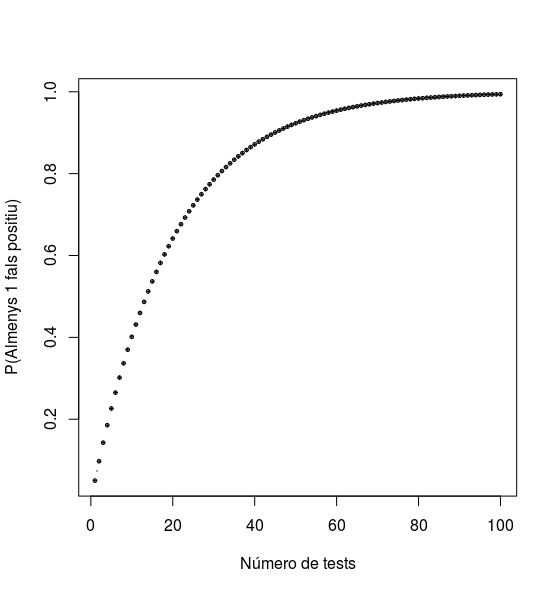
\includegraphics[scale=0.5]{FalsPositiu.png}
\captionof{figure}{Gràfic contraposant el nombre de tests amb la probabilitat d'obtenir almenys 1 fals positiu. S'observa un increment en la probabilitat quan augmenta el nombre de tests.}
\end{center}
En el nostre estudi es important tenir clar aquest problema, ja que si tenim molts gens, i no apliquem una correcció, podem caure en l'error d'afirmar que un gen s'expressa diferencialment quan realment no ho fa.
\subsubsection{False discovery Rate}
%http://www.gs.washington.edu/academics/courses/akey/56008/lecture/lecture10.pdf
%https://rpubs.com/Joaquin_AR/236898
Existeixen molts mètodes per corregir el problema de la multiplicitat de contrastos. El més simple és el mètode de Bonferroni, on cada p valor es multiplica pel nombre de tests realitzats (acotant la probabilitat màxima a 1). És un mètode molt conservador i no és el més indicat per al nostre cas d'estudi.
Per a escenaris de large-scale multiple testing com els estudis de genòmica, els quals es realitzen milers de test de forma simultània, el resultat d'aquests mètodes és massa conservador i impedeix que es detectin diferències reals. Una alternativa és controlar el false discovery rate.
\\

El false discovery rate ($FDR$) es defineix com la proporció esperada de falsos positius d'entre tots els tests considerats com significatius. L'objectiu de controlar el false discovery rate es establir un límit de significació per a un conjunt de tests tal que, d'entre tots els tests considerats com significatius, la proporció d'hipòtesis nul·les (falsos positius) no superin un determinat valor.
Un altre avantatge afegit és la seva fàcil interpretació, per exemple, si un estudi publica resultats estadísticament significatius per a un $FDR$ del 10$\%$, el lector té la seguretat que, com a màxim, un 10$\%$ dels resultats considerats com a significatius són realment falsos positius.
\\
La primera aproximació per controlar el FDR va ser descrita per Benjamini $\%$ Hochberg en 1995. D'acord amb la seva publicació si es desitja controlar que en un estudi amb $n$ comparacions el $FDR$ no superi un percentatge $d$ hem de:

\begin{itemize}
\item Ordenar els $n$ tests de menor a major $pvalor$ ($p_{1}$,$p_{2}$,... $p_n$).
\item Es defineix $k$ com l'última posició per la qual es compleix que $p_i \leq d\frac{i}{n}$.
\item Es consideren significatius tots els $pvalors$ fins a la posició $k$ ($p_{1}$,$p_{2}$,... $p_k$).

\end{itemize}

El mètode proposat per Benjamini $\&$ Hochberg assumeix a l'hora d'estimar el nombre d'hipòtesis nul·les erròniament considerades falses, que totes les hipòtesis nul·les són certes. Com a conseqüència, l'estimació del $FDR$ està inflada i és un mètode conservador. Per poder veure l'afectació d'utilitzar un mètode com Bonferroni o utilitzar el métode Benjamini $\&$ Hochberg, tenim la següent taula d'exemple:
\\
\begin{table}[ht]
\centering
\begin{tabular}{rrrr}
\hline
& Pvalor & Bonferroni & Benjamini$\&$Hochberg \\
\hline
1 & 0.0010 & 0.0550 & 0.0037 \\
2 & 0.0020 & 0.11 & 0.0069 \\
3 & 1 & 1 & 1 \\
4 & 0.0010 & 0.0550 & 0.0037 \\
5 & 0.0010 & 0.0550 & 0.0037 \\
6 & 0.0010 & 0.0550 & 0.0037 \\
7 & 0.25 & 1 & 0.3929 \\
8 & 0.48 & 1 & 0.6286 \\
9 & 0.09 & 1 & 0.1650 \\
10 & 0.51 & 1 & 0.6523 \\
\hline
\end{tabular}
\caption{A l'exemple de la taula hi ha una columna amb les $pvalors$ sense corregir, un altre amb la correcció de Bonferroni i per últim una amb la correcció proposada per Benjamini$\&$Hochberg, per a un total de 55 $pvalors$ (Encara que només es mostren els 10 primers). Observem que Bonferroni és un mètode molt més conservador i cap $pvalor$ és significatiu. (Dels 55 $pvalors$, 0 són significatius amb Bonferroni). En canvi, amb el mètode de Benjamini$\&$Hochberg, observem que del total de $pvalors$, hi ha 26 significatius.(En aquest cas hem fixat un $\alpha=0.05$ i un $FDR=0.05$) }
\end{table}

A l'hora de decidir quin tipus de correcció aplicar, és important utilitzar un mètode adequat per tal d'obtenir resultats més acurats. En els estudis exploratoris és d'esperar que la proporció d'hipòtesis nul·les falses, és a dir, tests que són realment significatius, sigui alta. Per tant, mètodes que només depenen del nombre de tests no són els més potents per aquest tipus d'estudis, com hem vist anteriorment.

\subsection{Post hoc testing: Tukey}
\subsection{Anàlisi de components principals}
\subsection{Heatmap}
%%% RESULTS
\section{Cas d'estudi:Resultats del protocol d'anàlisi}
\subsection{Resultats}
\subsubsection{Tractament de les dades}
\subsubsection{Anàlisi de la variància (ANOVA)}
\subsubsection{Correcció per multiplicitat de contrastos}
\subsubsection{Anàlisi de components principals}
\subsubsection{Heatmap anàlisi}
\subsection{Conclusions}
%%Shiny
\section{TL3P: Aplicatiu Web amb el paquet Shiny de R}
\subsection{Introducció a Shiny}
An alternative method to create web-based teaching tool applications is provided by Shiny
(Chang, Cheng, Allaire, Xie $\&$ McPherson, 2015), a recent technology created by RStudio.
Shiny is a web application framework for R (R Core Team, 2015) that only requires knowledge
in the R programming language. It is not uncommon for instructors to build their
own teaching tools via scripts written in R and, as we will show, it is not difficult to convert
existing R scripts into Shiny applications, known simply as ‘Shiny apps’. With Shiny,
instructors can build a teaching tool that is interactive, dynamic, user-friendly, visually
appealing, and, with similar functionality to Java/Javascript applets; the only requirement
is some familiarity in R.
\subsubsection{Estructura de l'aplicatiu}
\subsubsection{Gestió per mitjà de repositoris Github}
\subsection{Funcionalitats de l'aplicació}
\subsection{Desenvolupament i futures versions}
%Bibliografia
\section{Bibliografia}
%%Appendix



\end{document}
